\chapter{系统结果与分析}
\label{result}

本章节将会首先总结系统功能,然后简单对系统的性能、交互方式、虚实融合效果三部分进行最终结果的分析。

\section{系统功能汇总}
本系统实现了一个可以获得真实触感的增强现实应用。其中服务器使用LibISR物体追踪工具,以及Kinect 2深度摄像机,实现对已知模型的物体进行追踪。

前端交互系统提供了注册、登陆、编著、交互四部分。编著系统提供了添加和移动物体、编辑物体、编辑实验场景、编辑实验流程和提示板、编辑已有实现等功能。交互系统通过和物体追踪系统进行网络交互,对单个创建的物体进行追踪、标定、显示,并且提供使用样例。

用户可以通过本应用,在手机或电脑端编著实验,通过手机摄像头对场景中的真实物体进行追踪,并显示虚拟信息,实现有真实触感的增强现实应用。

\section{性能分析}

首先对物体追踪引擎仅进行追踪的时候的性能进行测试。物体追踪引擎运行环境为Intel Core i7 4790K处理器以及Nvidia GeForce GTX 980的显卡。

测试在仅进行单个物体追踪,没有网络传输时服务器端的性能。其中为了准确仅计算了ISRCoreEngine中处理每一帧图像的时间,追踪结果如图\ref{fig:fps}所示,其中从左至右分别为开始追踪前、未找到追踪物体、追踪物体静止、追踪物体运动四种情况。帧率统计结果如图\ref{fig:fps}所示,其中横坐标为每一帧,纵坐标为对应的帧率。

\begin{figure}[!htp]
  \centering
  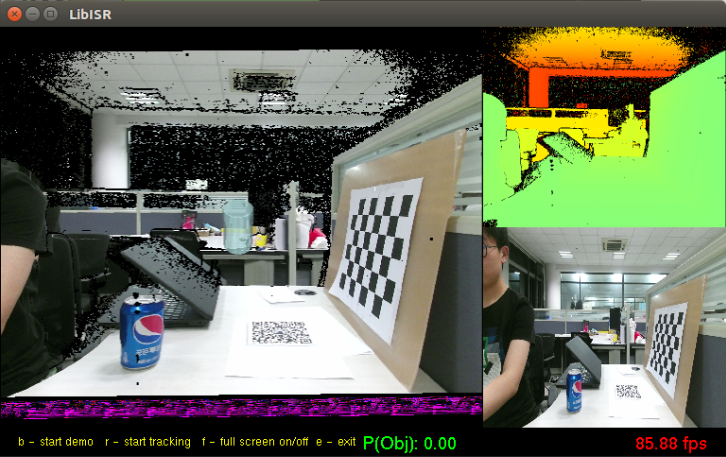
\includegraphics[width=6cm]{figure/beforeT.png}
  \hspace{1cm}
    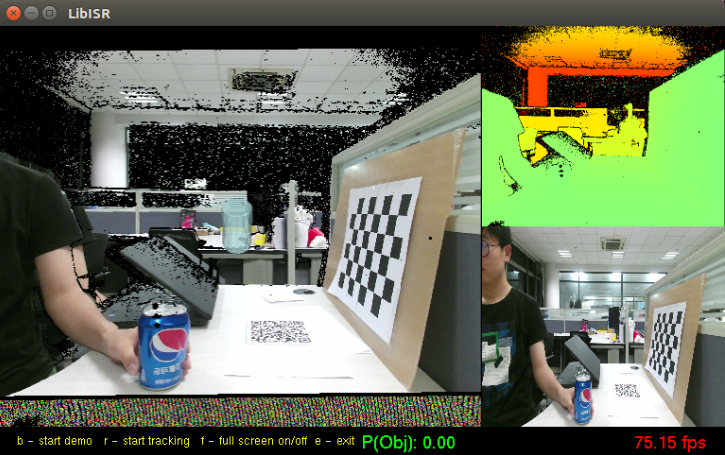
\includegraphics[width=6cm]{figure/noT.png}
    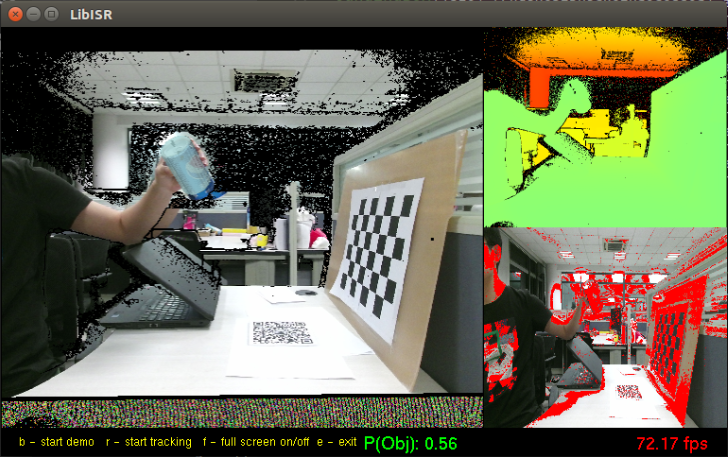
\includegraphics[width=6cm]{figure/staticT.png}
  \hspace{1cm}
  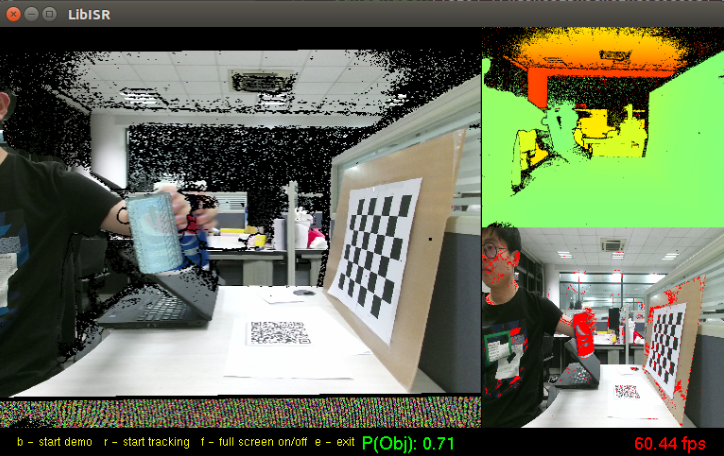
\includegraphics[width=6cm]{figure/movingT.png}
  \bicaption[物体追踪不同状态截图]
    {物体追踪不同状态截图}
    {The Screen-shots of Tracing Object in Different Situations}
  \label{fig:SRR}
\end{figure}


\begin{figure}[!htp]
  \centering
  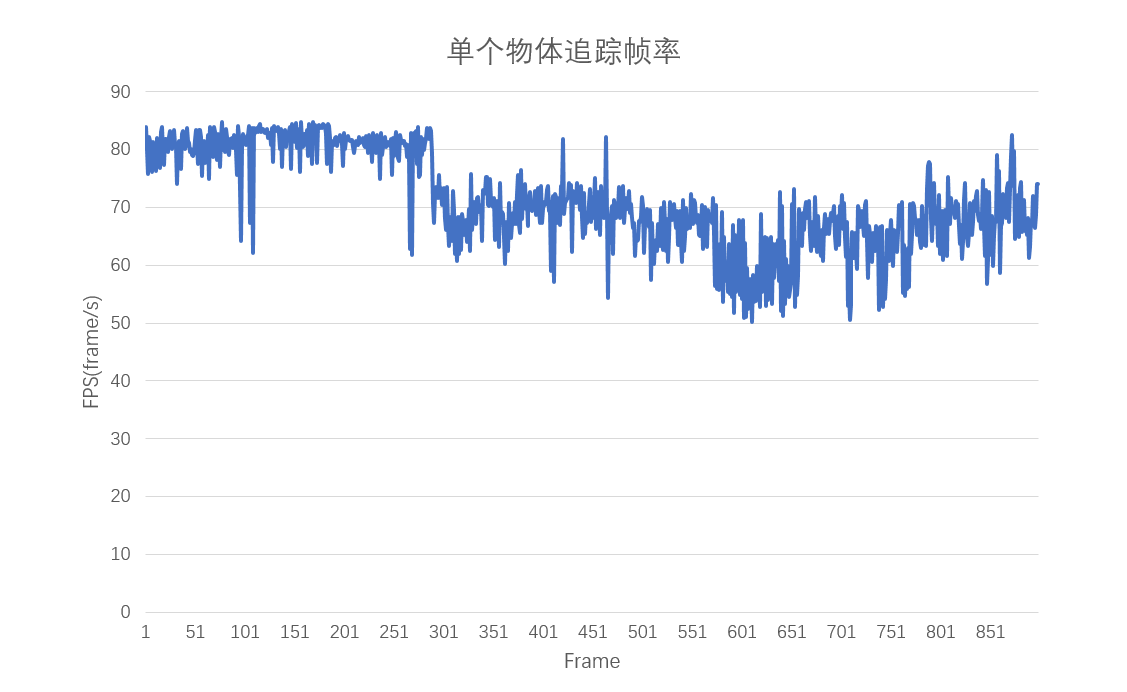
\includegraphics[width=10cm]{figure/fps.png}
  \bicaption[单个物体追踪帧-帧率折线图]
    {单个物体追踪帧-帧率折线图}
    {The Line Chart of Frame - Frame Per Second of Tracing Single Object }
 \label{fig:fps}
\end{figure}

从图中可以看出,在开始追踪之前,即仅测量从Kinect获取视频图像的性能,帧率约为80。从250帧左右开始追踪之后,帧率下降,当物体基本保持静止时或物体并没有被追踪到时,帧率约为70。当第550至650帧时,物体处于移动状态,帧率约为55帧。由此可见,帧率在追踪移动物体的时候性能消耗最大,但整体仍然满足60帧的性能需求。

之后在开启网络通信的情况下,检测客户端获取数据的速率,实际上也就是增强现实应用中物体运动姿态更新的频率。在程序中使用一个计数器,会在每次有数据接收的时候计数,然后每秒进行统计。客户端的运行环境为Intel Core i7 6500U处理器以及AMD Radeon R7 M370显卡。由于客户端和服务器传输数据通过代码保证同步,因此该数据也代表了服务器的数据发送速率。经过测试,网络传输保持在每秒25次,这很大程度上是由于网络传输本身,以及实现的同步收发机制所限制的。此外,也利用Unity中的Coroutine进行每秒统计项目的帧数计算帧率,项目的帧率则被Unity保持在60。

最后,也检测了在移动端应用接受数据的传输速率。手机使用HiSilicon Kirin 970处理器。此时网络通讯速率仍然为每秒25次,项目帧率被Unity锁在30,但是实际上并不影响使用体验。

\section{编著系统}
系统在PC端和安卓手机端都进行了安装,两者都可以完成预期的工作。

在使用手机应用进行实验编著时,用户可以顺利完成点击、拖动等操作,实现预期需求,例如图\ref{fig:authorRes}中展示的,实验器具和药品的添加和编辑,物体移动,实验环境的编辑,实验流程的编辑等。所有的交互方式与PC端保持一致,只需要用手指触摸代替鼠标点击。此外,通过用户试用反馈来看,在物体的创建、编辑等部分可以很快操作,但是流程编辑的部分则有些复杂。

\begin{figure}[!htp]
  \centering
  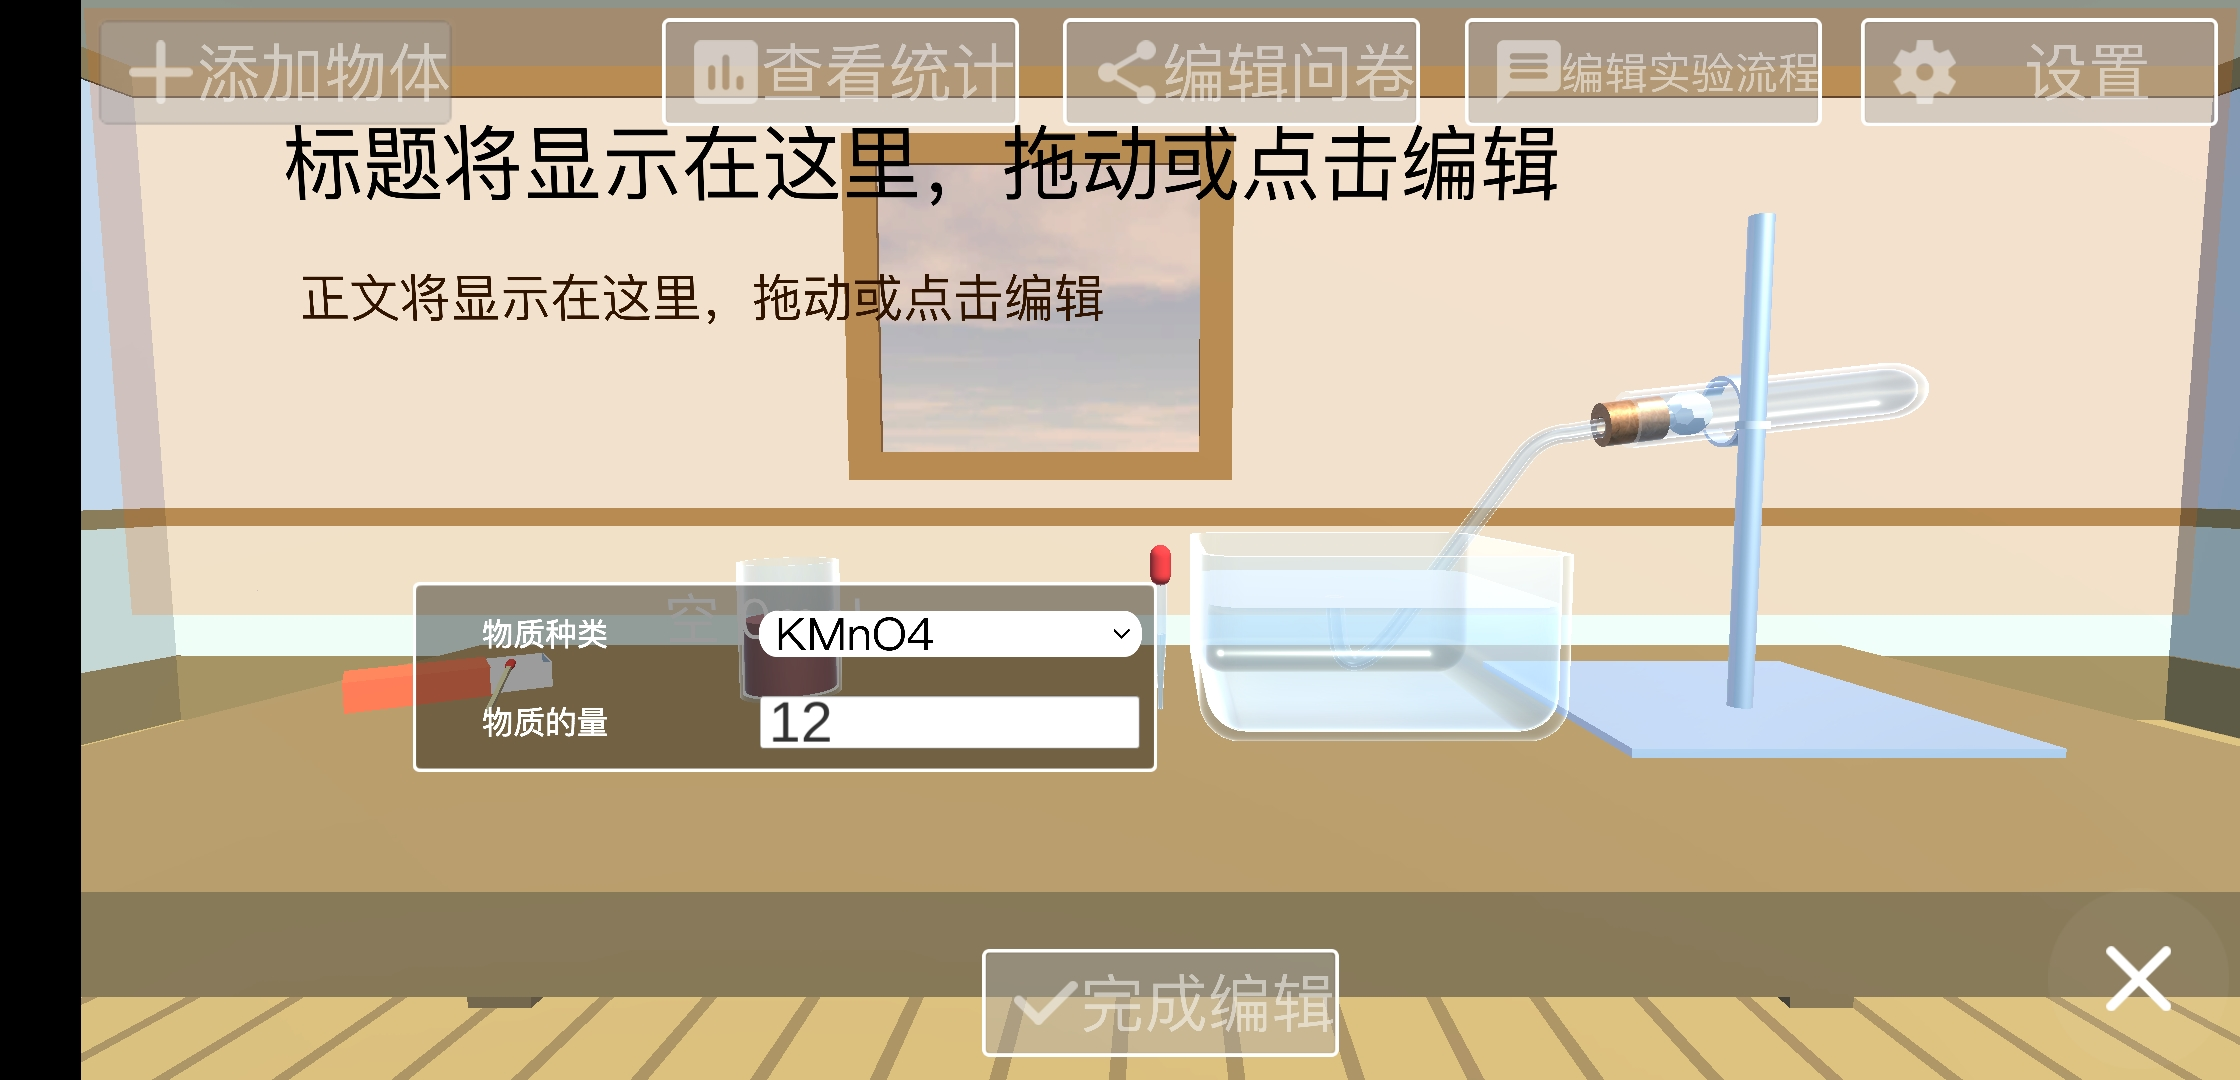
\includegraphics[width=6cm]{figure/objRes.jpg}
  \hspace{1cm}
    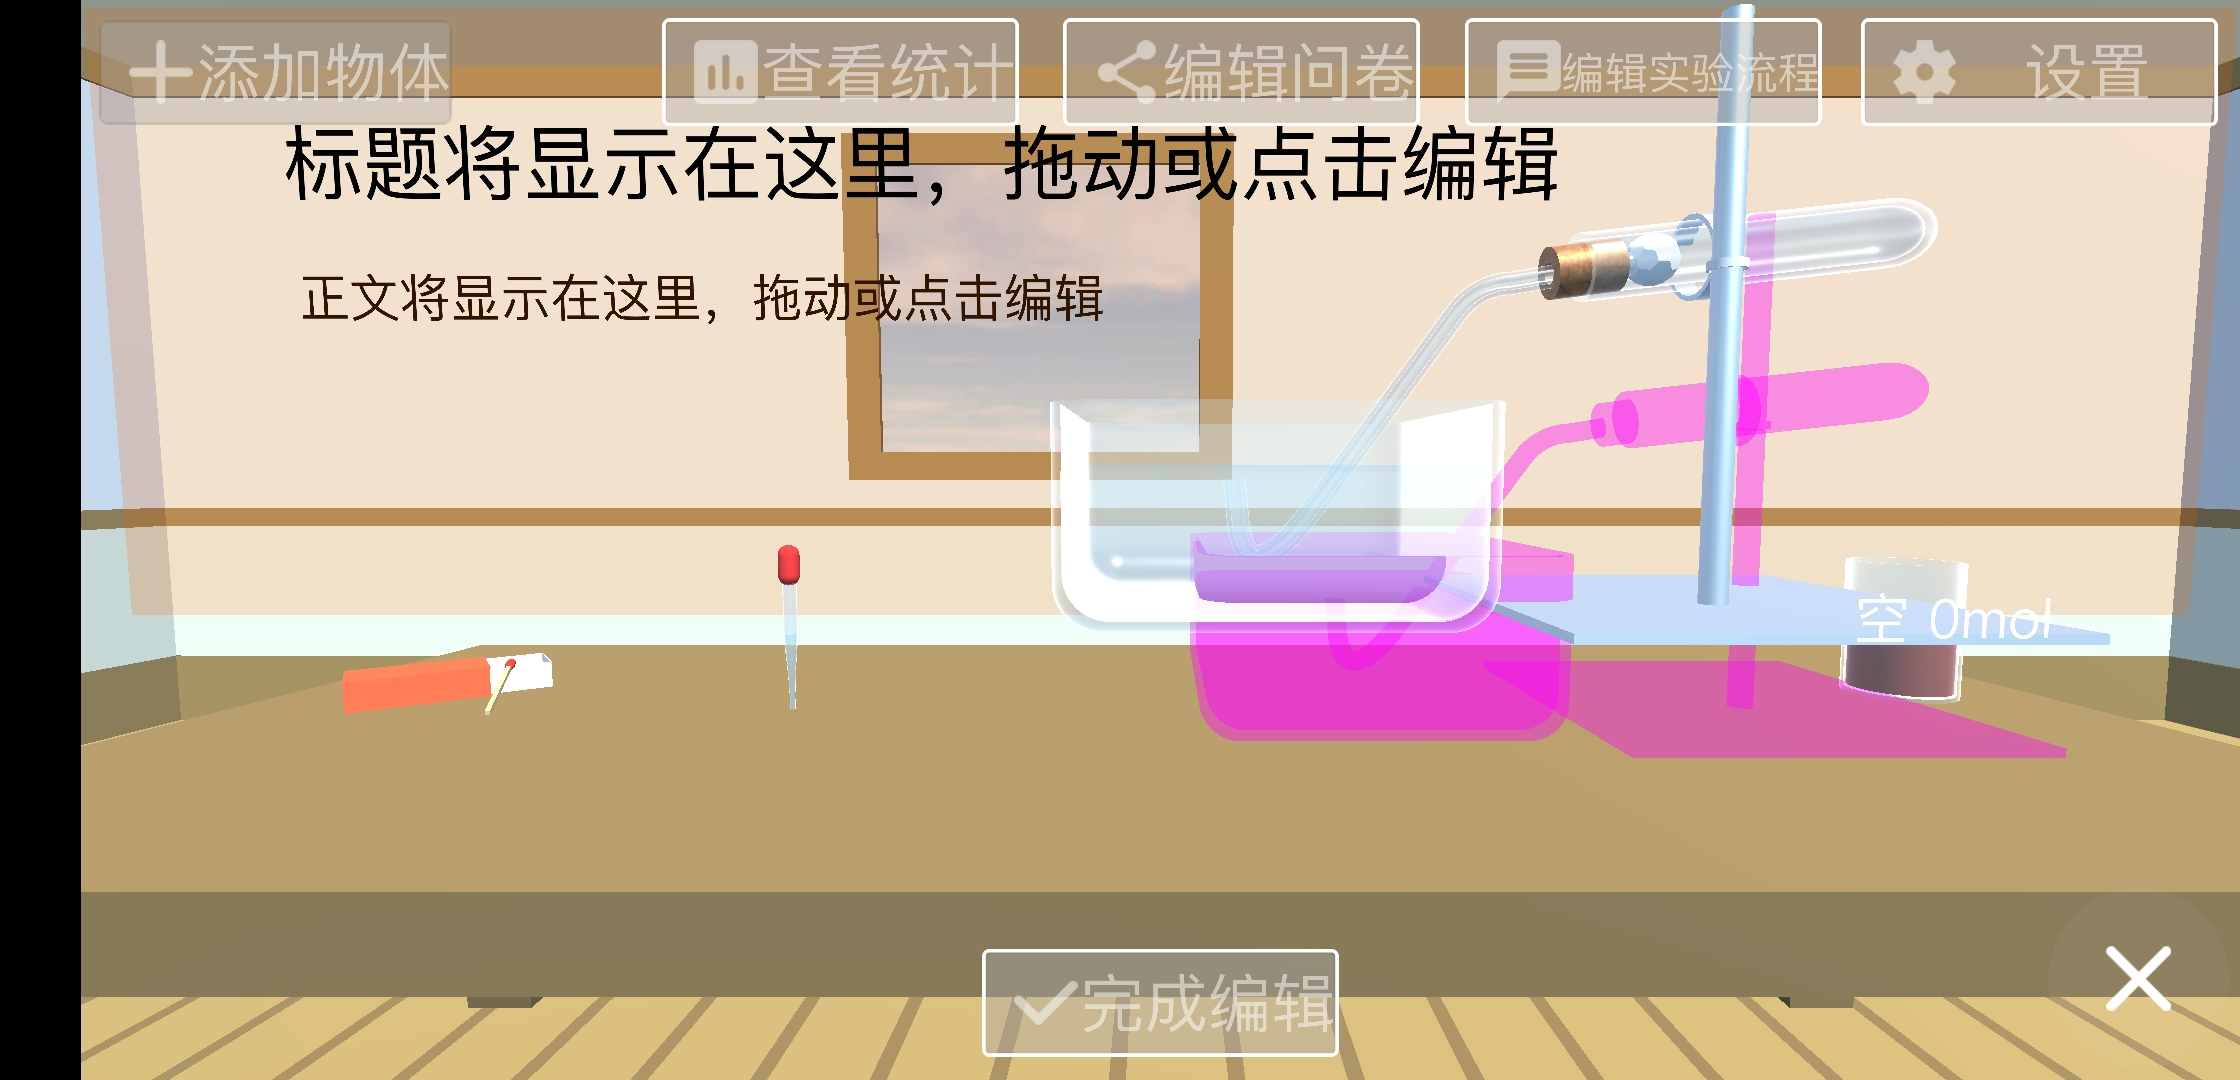
\includegraphics[width=6cm]{figure/movingRes.jpg}
    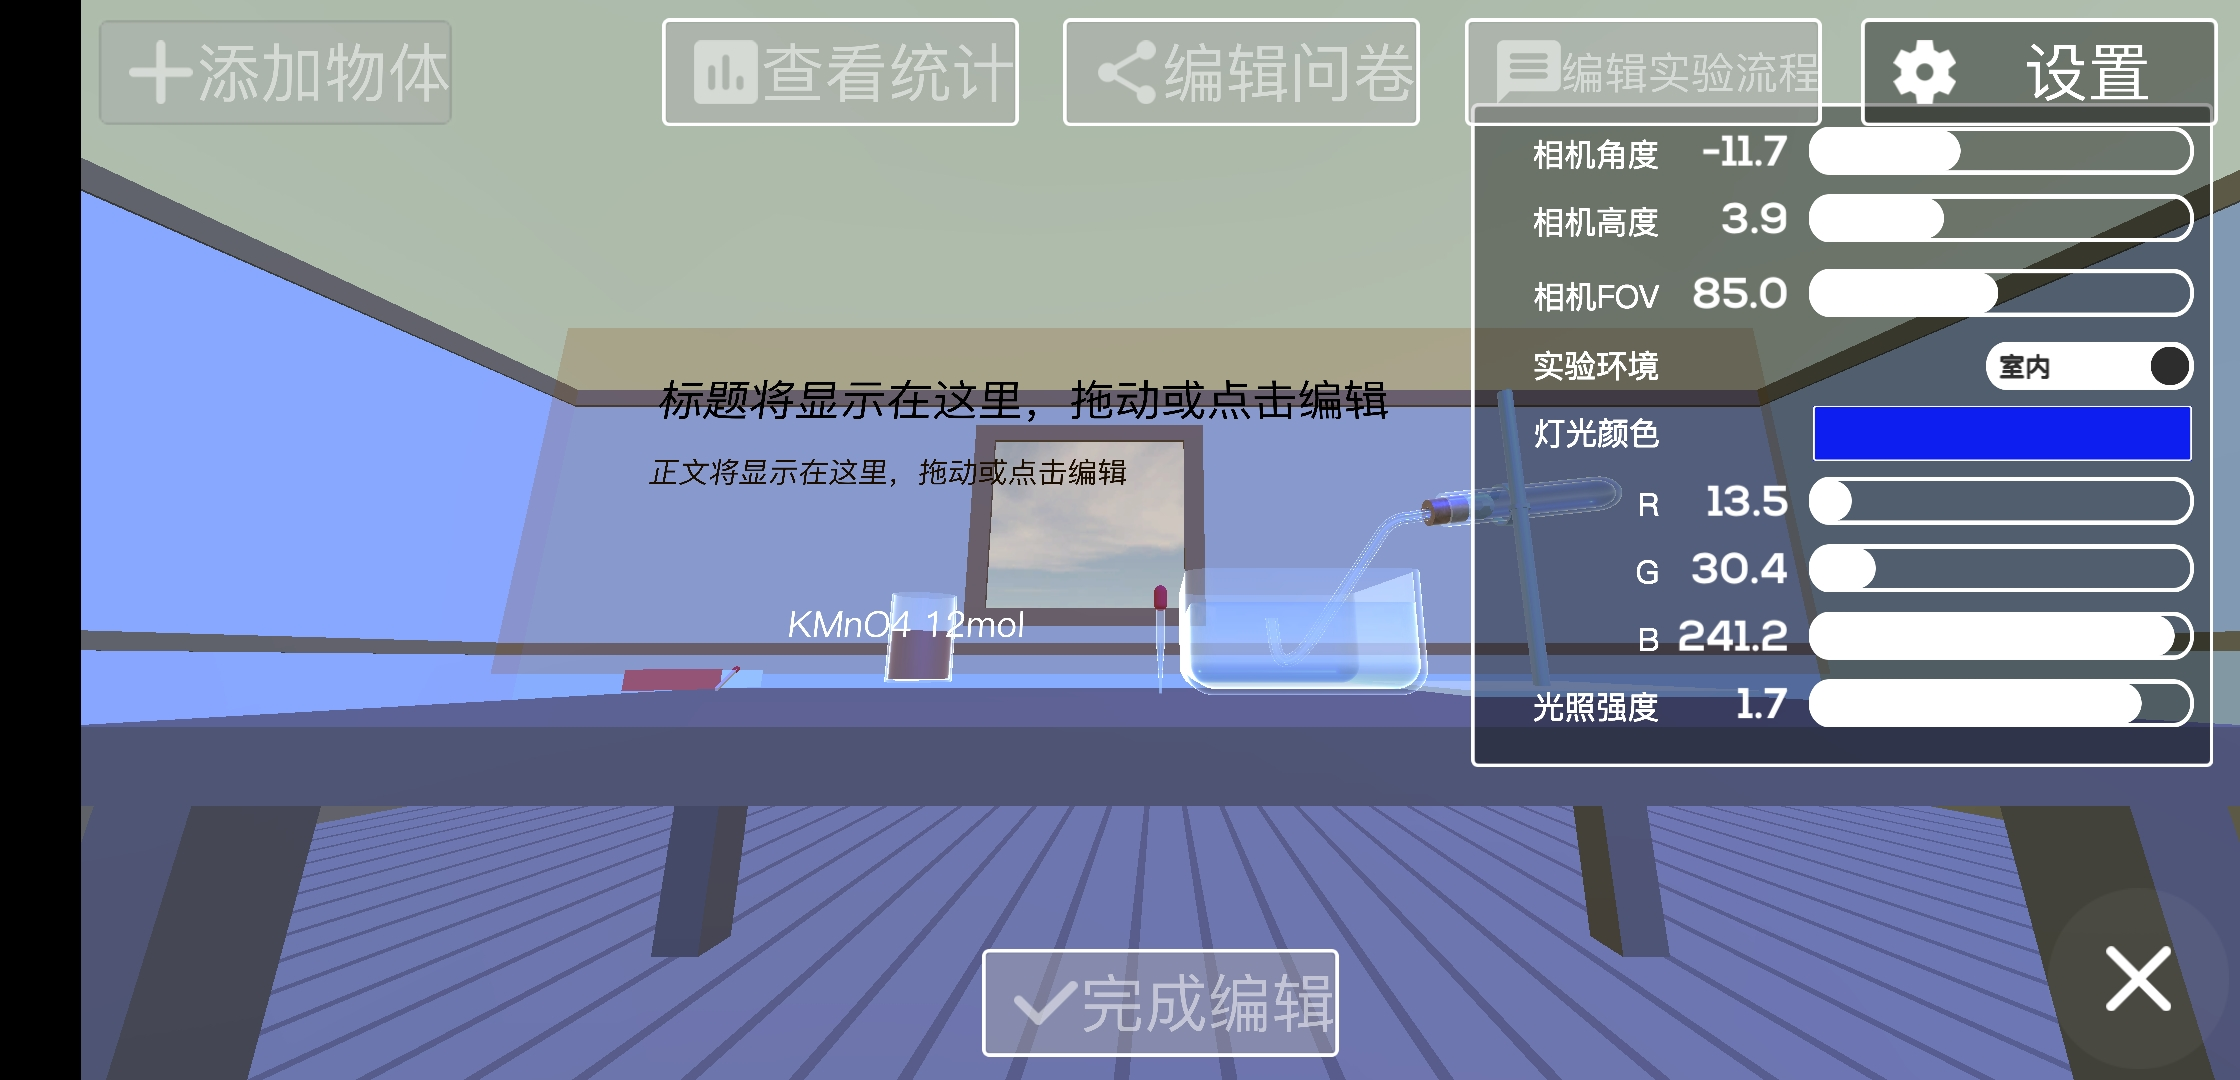
\includegraphics[width=6cm]{figure/envirRes.jpg}
  \hspace{1cm}
  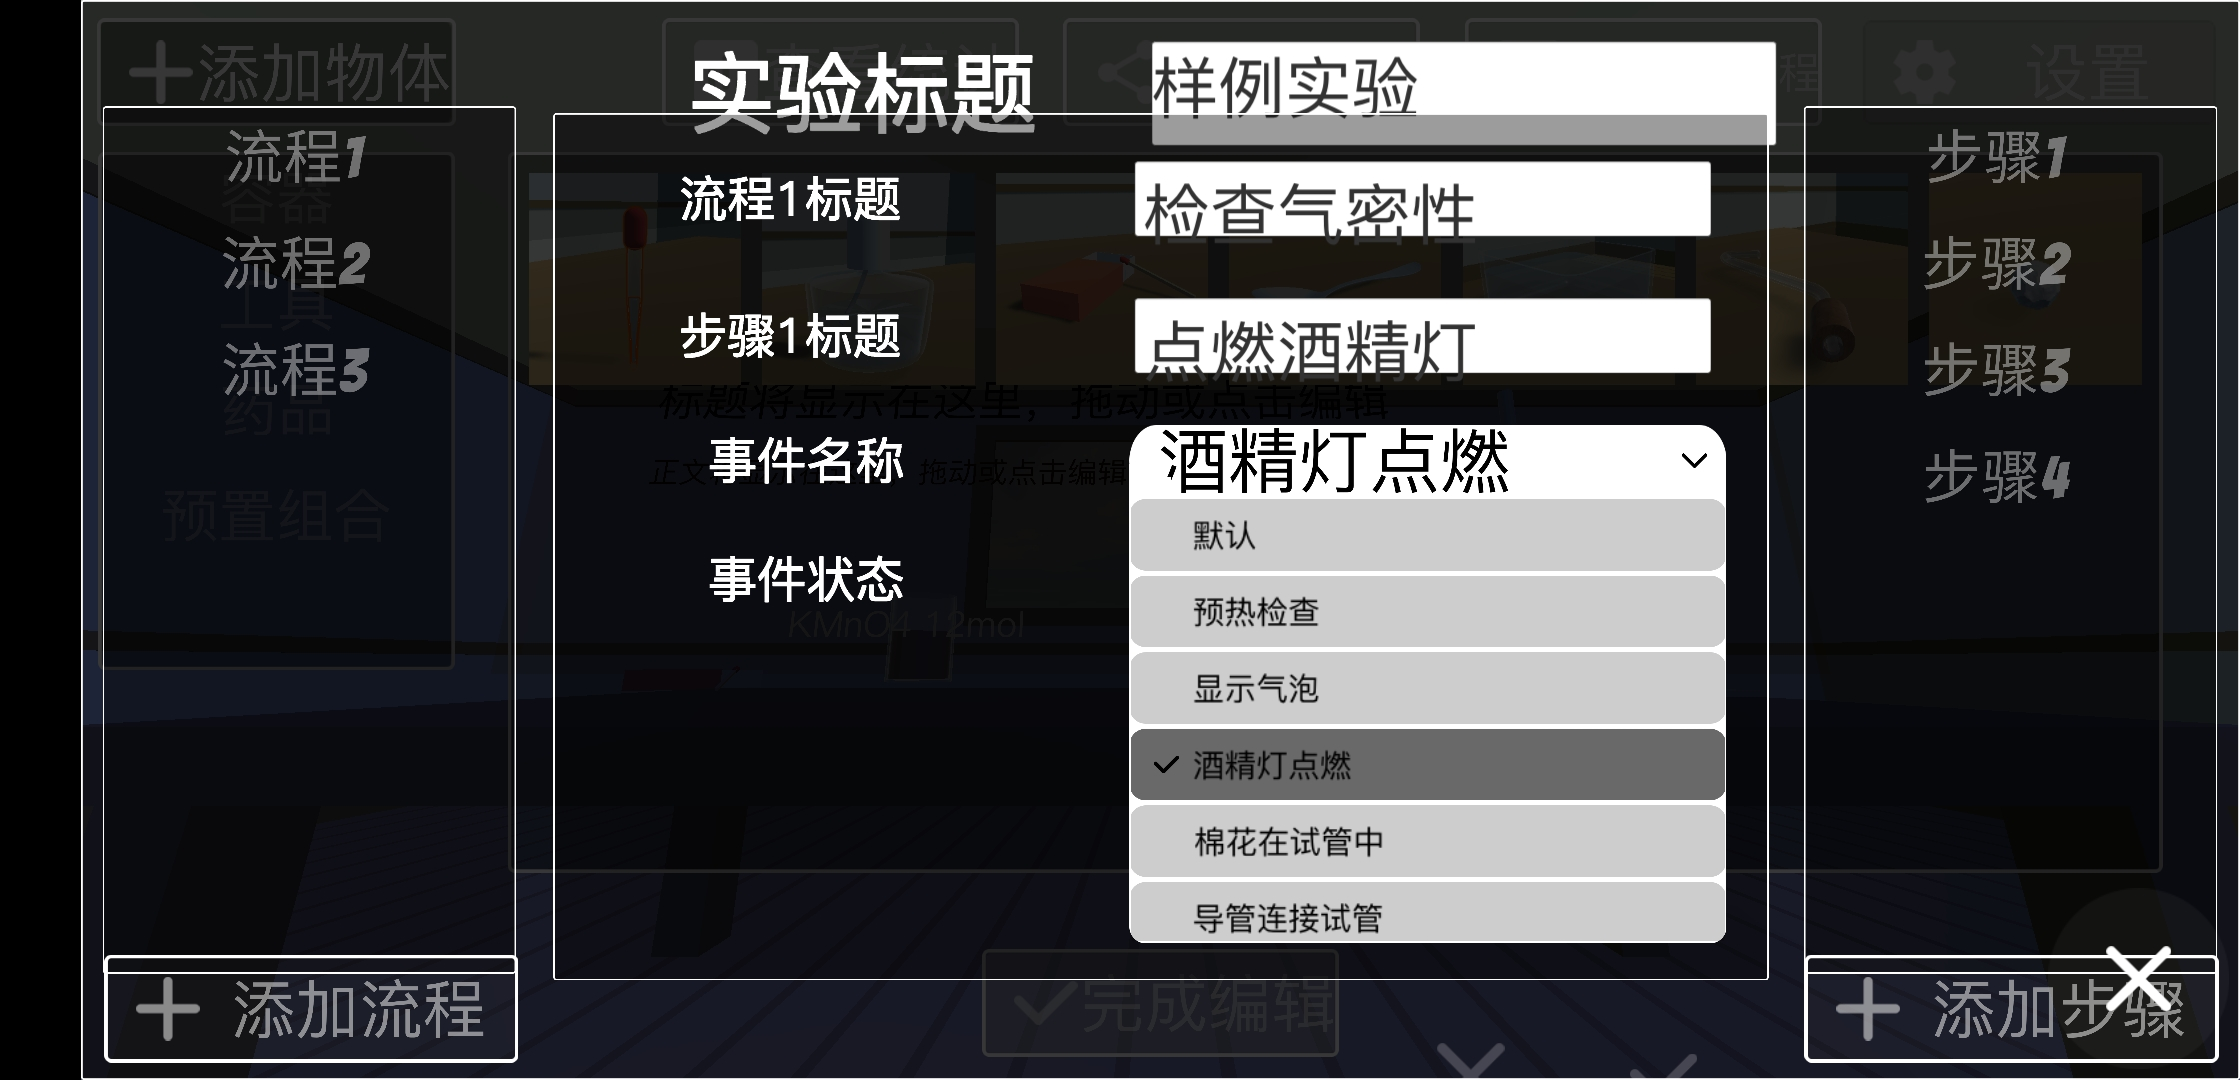
\includegraphics[width=6cm]{figure/procedureRes.jpg}
  \bicaption[手机端编著系统截图]
    {手机端编著系统截图}
    {The Screen-shots of Authoring System on Mobile Device}
 \label{fig:authorRes}
\end{figure}

系统目前支持了工具、容器、药品、预置组合四大类物品,包括酒精灯、集气瓶、火柴、水槽、烧杯等高中化学实验需要的器材,以及铁、高锰酸钾、稀盐酸等高中化学实验常用药品。通过组合所有支持的器材和药品,用户可以编辑出完整的高锰酸钾制氧气的实验。

\begin{figure}[!htp]
  \centering
  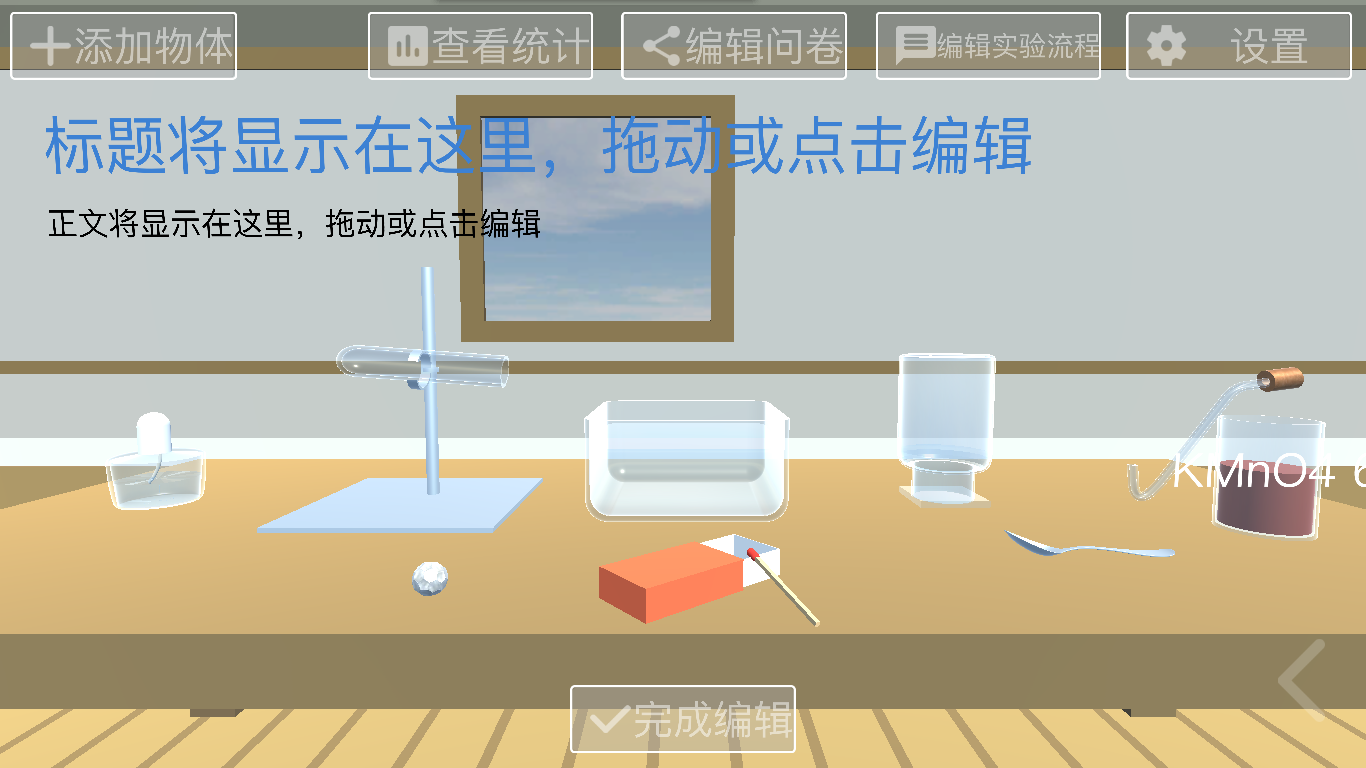
\includegraphics[width=12cm]{figure/Kmno4res.png}
  \bicaption[编著高锰酸钾制氧气实验截图]
    {编著高锰酸钾制氧气实验截图}
    {The Screen-shot of Authoring the Oxygen Production Experiment with $KMnO_4$}
 \label{fig:authorRes}
\end{figure}


\section{虚实融合效果分析}
在增强现实页面,用户可以通过手机向服务器发送指令,开始追踪,并且经过标定后,将虚拟物体与真实物体重合并且同步移动。在这个过程中,用户需要用手机拍摄到二维码,之后可以移动物体并观察手机中的虚拟图像。增强现实应用的用户界面如图\ref{fig:mAR}所示,此时还未开始追踪,物体处于初始状态。

\begin{figure}[!htp]
  \centering
  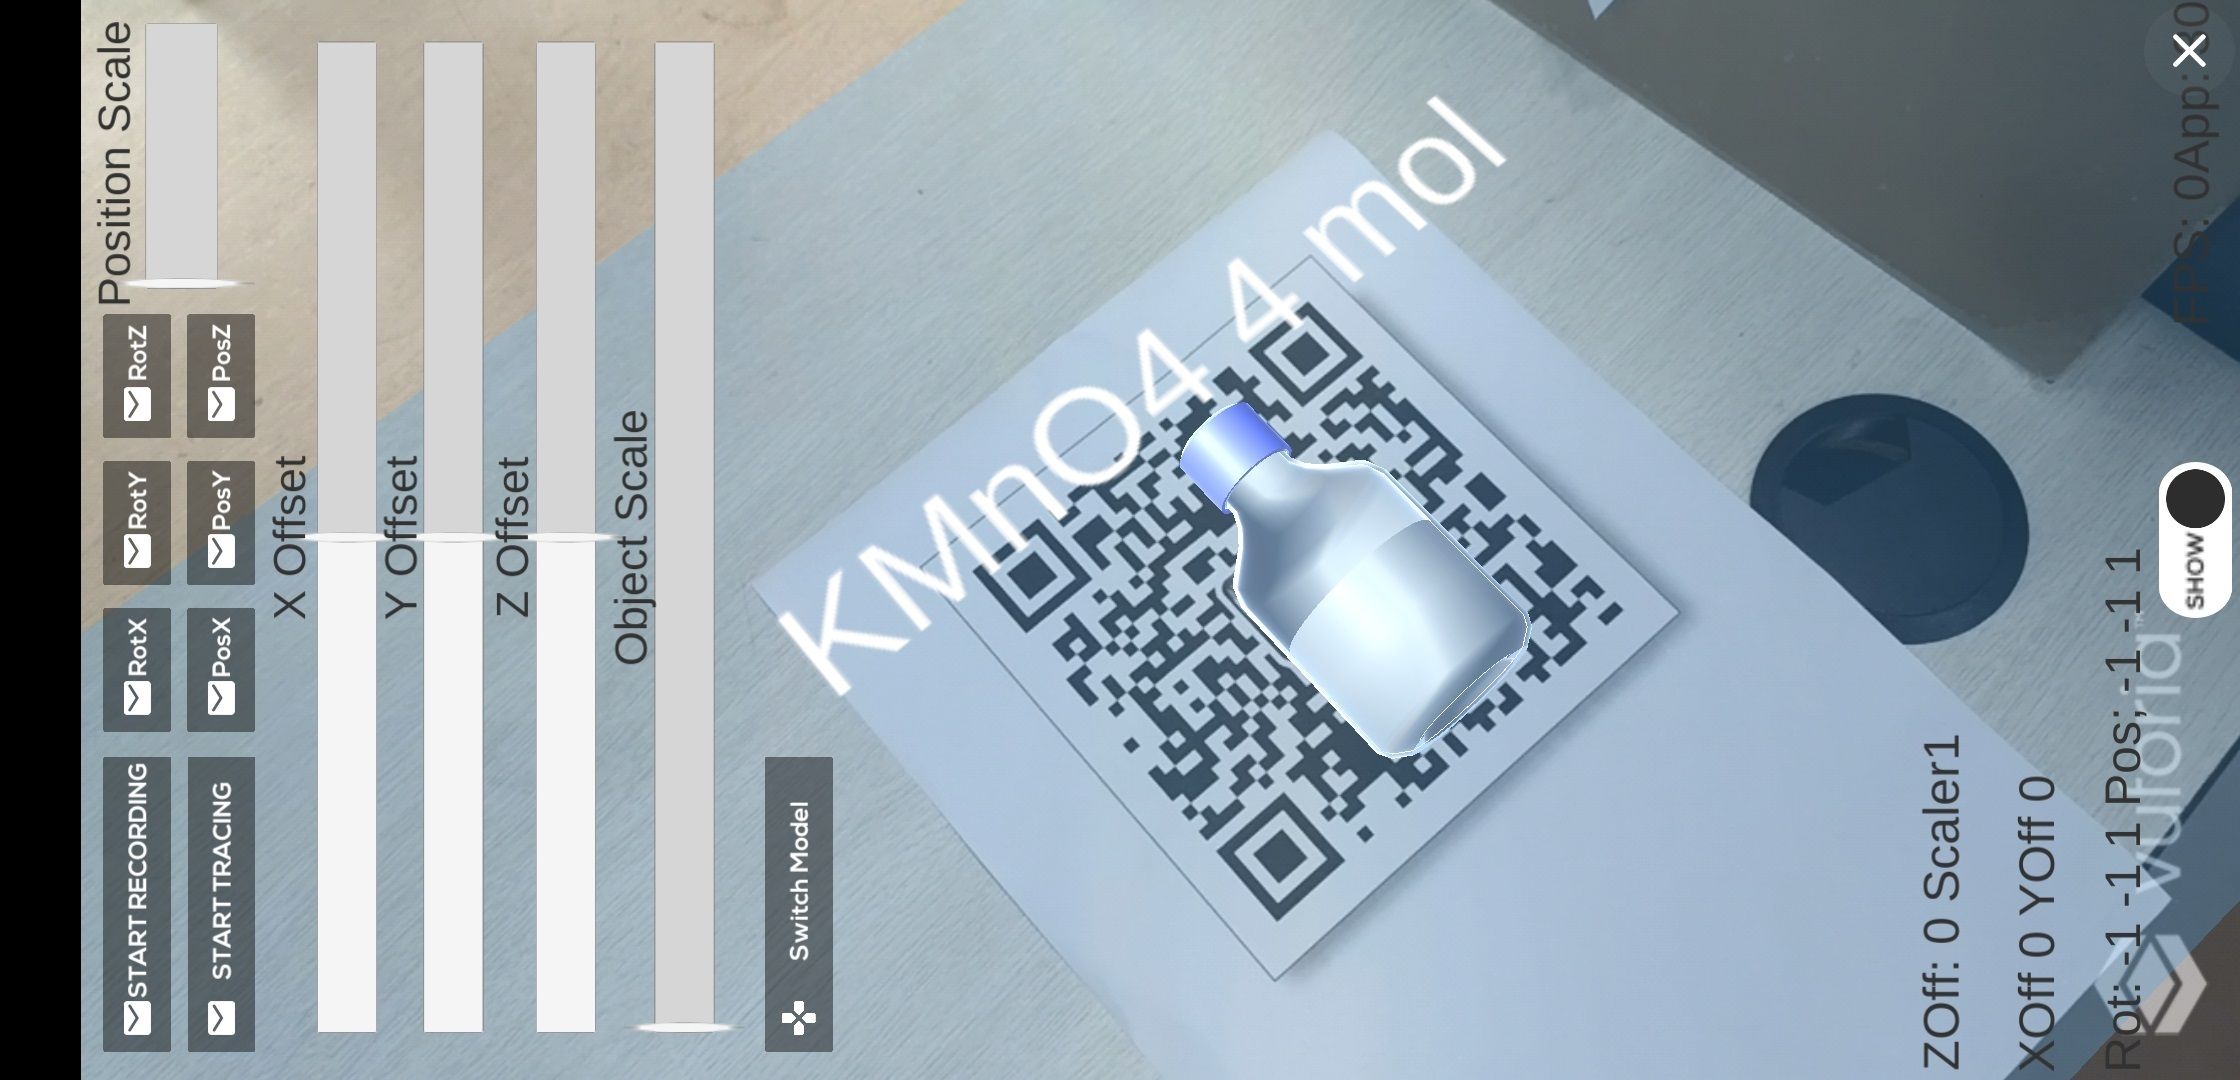
\includegraphics[width=12cm]{figure/ARui.jpg}
  \bicaption[增强现实应用用户接口截图]
    {增强现实应用用户接口截图}
    {The Screen-shot of User Interface in AR application }
 \label{fig:ARUI}
\end{figure}

图中的UI控件用于辅助用户进行标定,包括物体的大小、坐标映射关系等等。它们已经确定,不再需要用户修改,用户只需要根据使用情景修改xyz三个方向上的偏移量就可以了,相关控件可以在标定完成之后隐藏。标定完成后,用户可以在增强现实场景中看到在编著系统中编著好的的实验。
\begin{figure}[!htp]
  \centering
  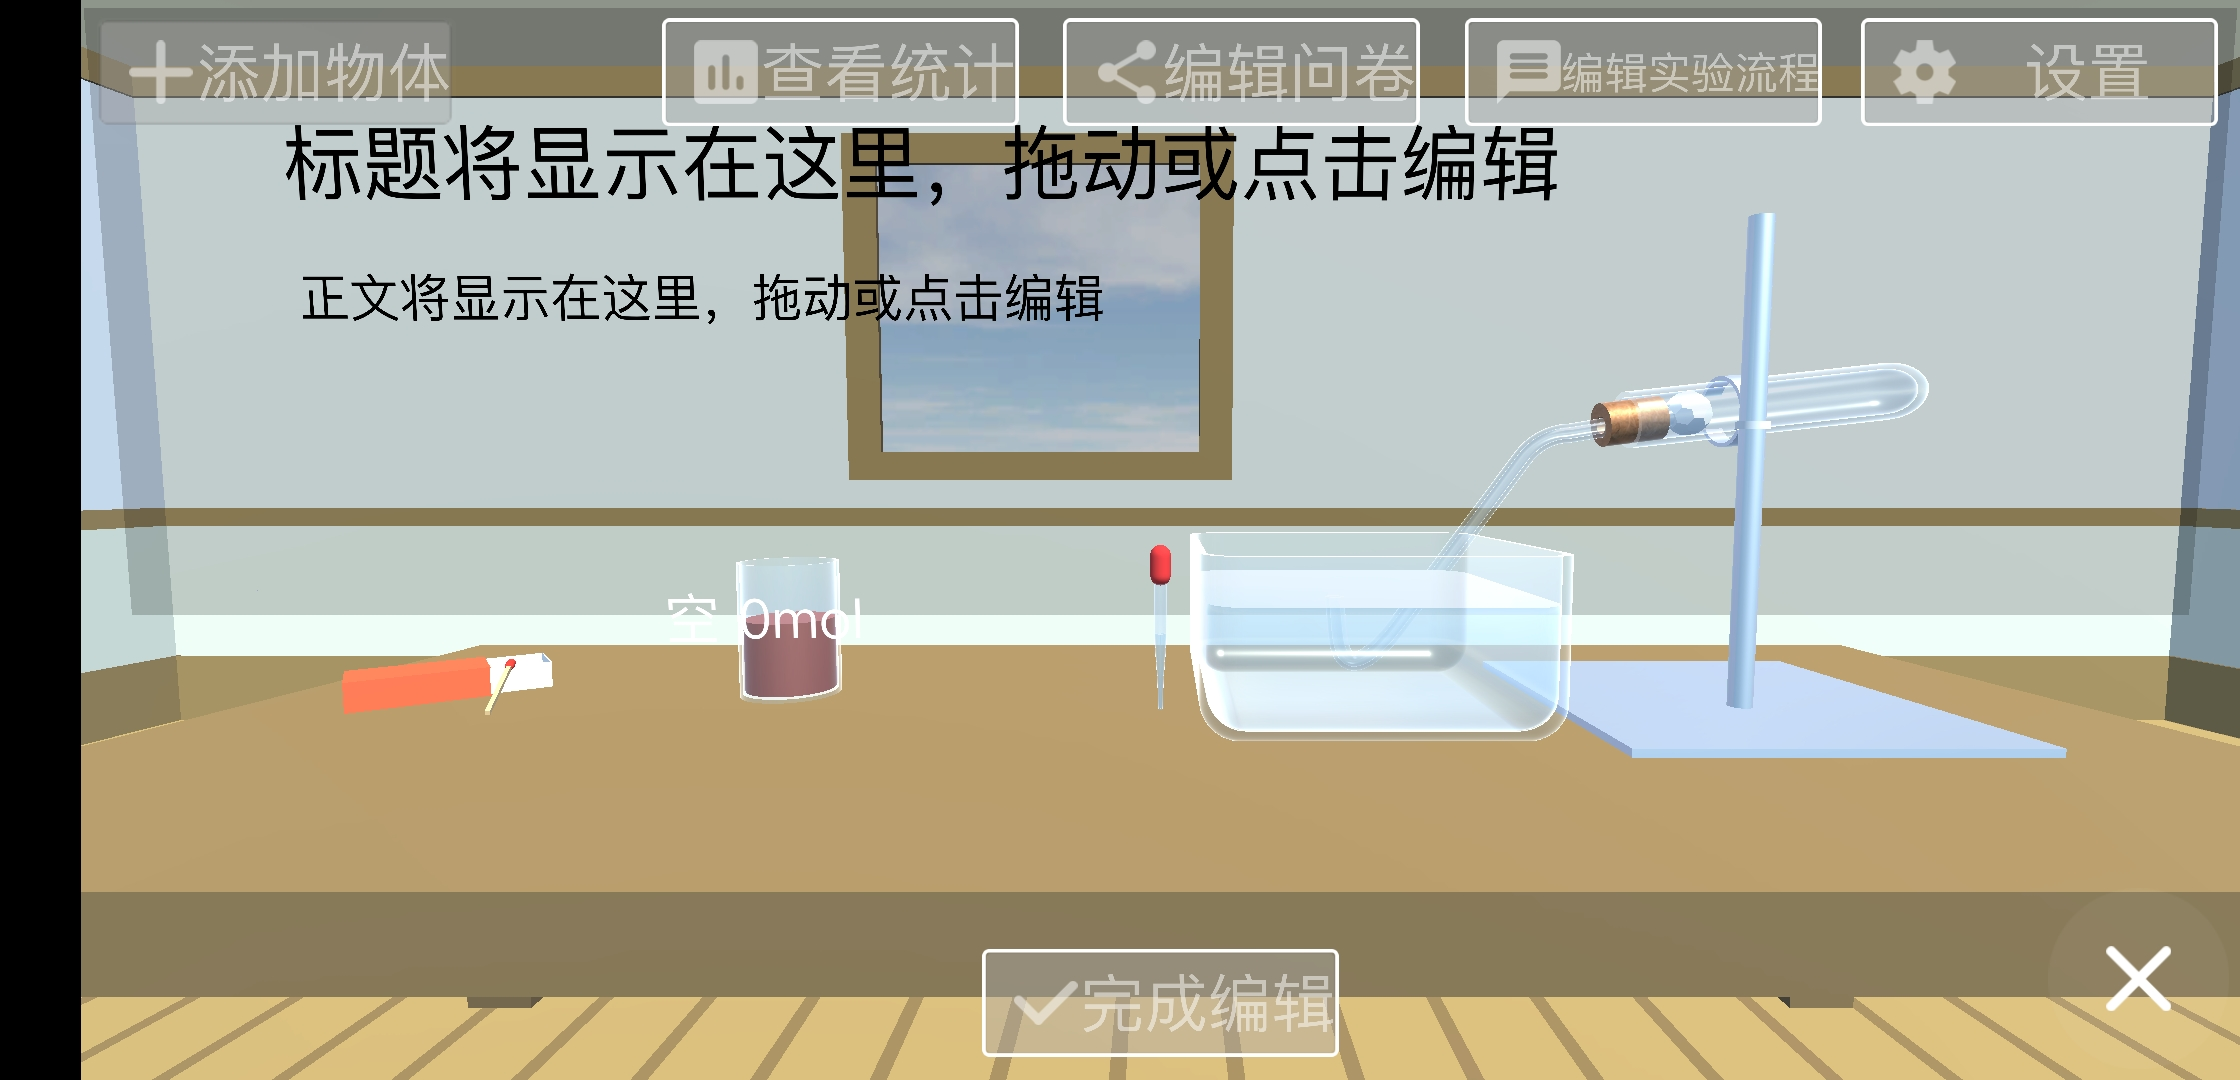
\includegraphics[width=6cm]{figure/authorRes.jpg}
    \hspace{1cm}
  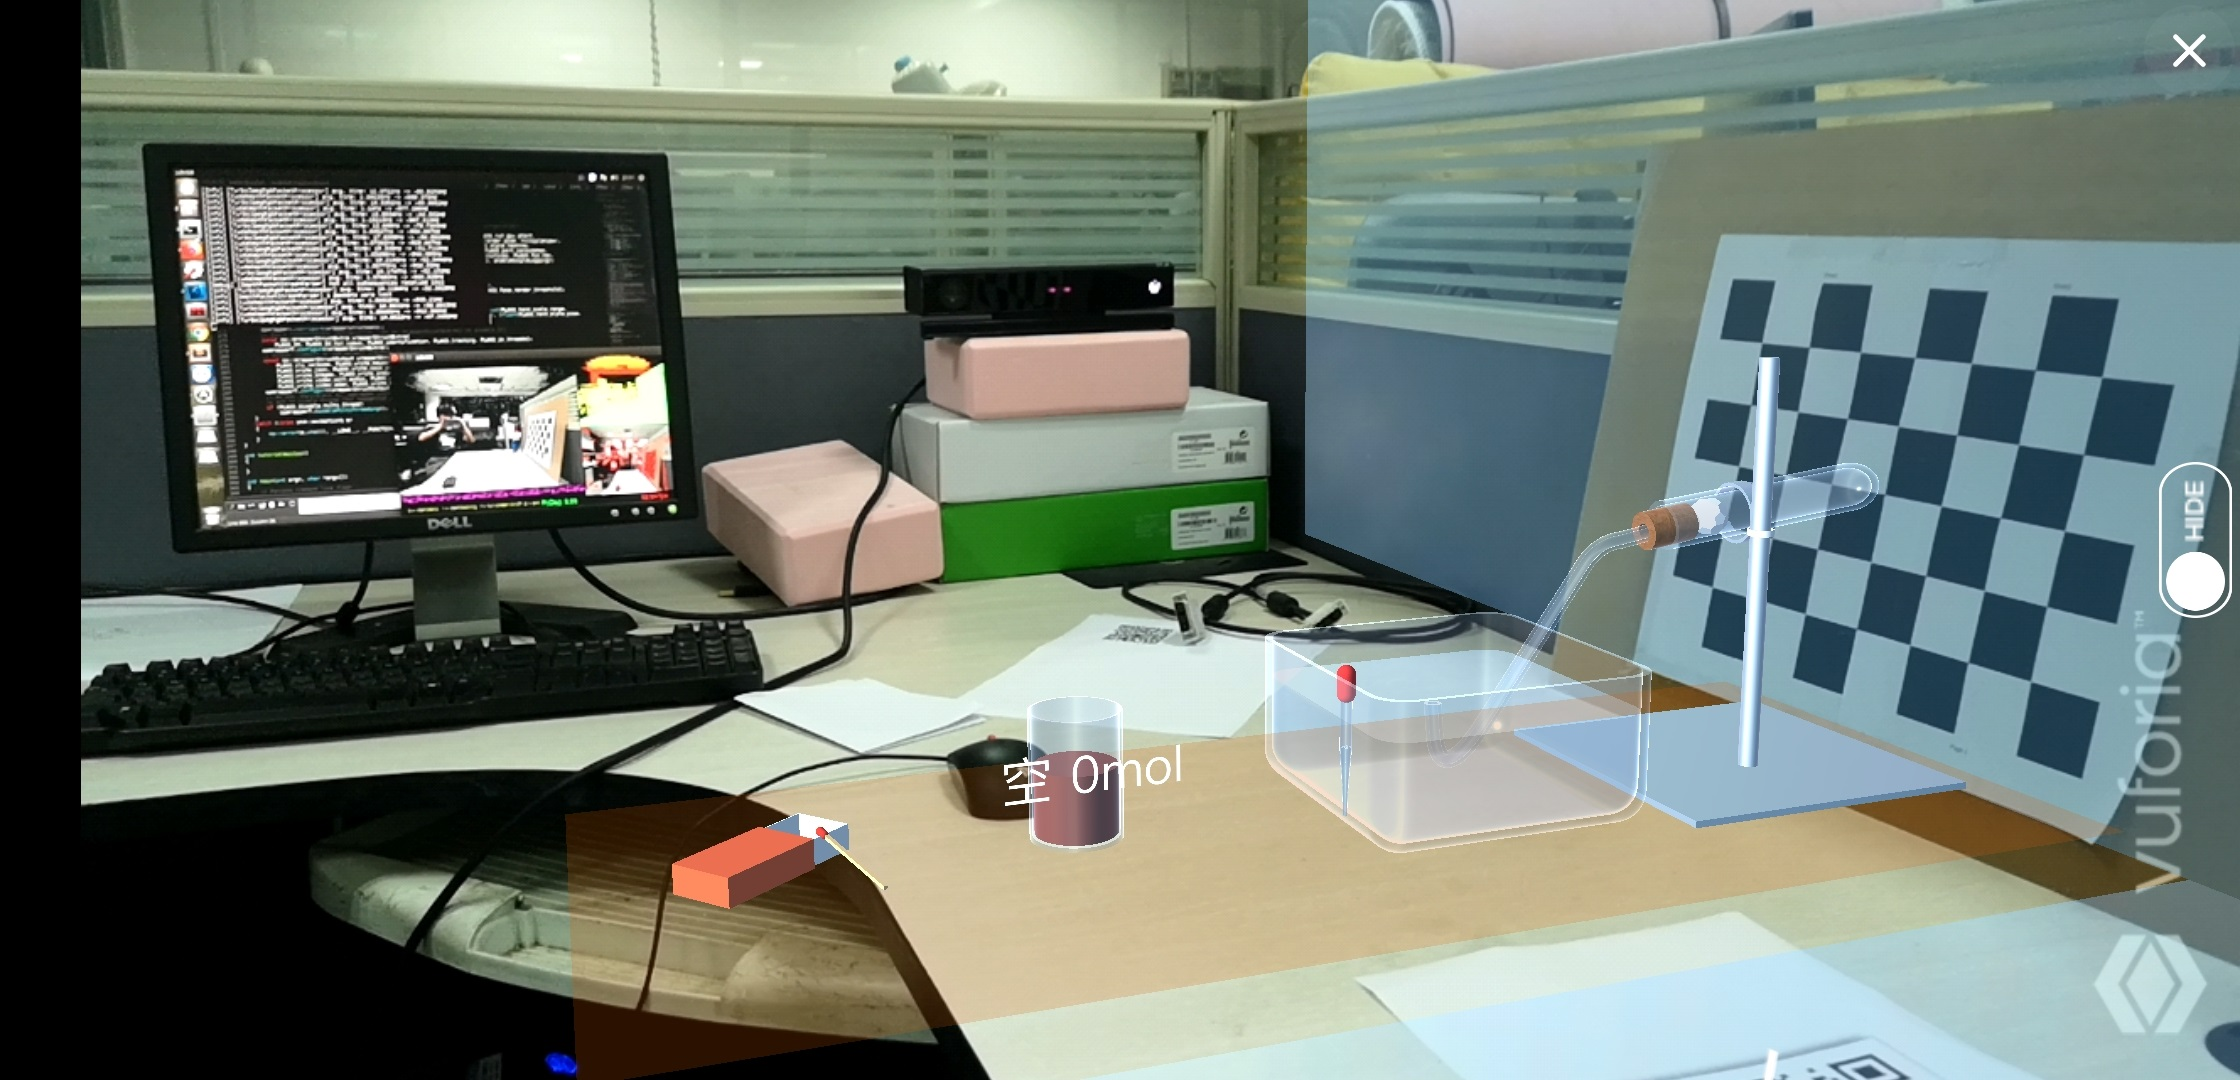
\includegraphics[width=6cm]{figure/table.jpg}
  \bicaption[编著系统与增强现实系统实验对比图]
    {编著系统与增强现实系统实验对比图}
    {The Comparison Figure of Experiments in Authoring System and AR Application}
 \label{fig:comp}
\end{figure}

之后用户就可以在实验场景中移动物体进行虚实融合了。用户需要首先使用图\ref{fig:ARUI}中的按钮向服务器发送指令,之后服务器就会开始对物体进行追踪,并将追踪结果实时显示在增强现实应用中。被追踪的物体还会显示用户在编著系统中输入的物质种类以及量,这样的虚拟信息结合了增强现实的特性。

\begin{figure}[!htp]
  \centering
  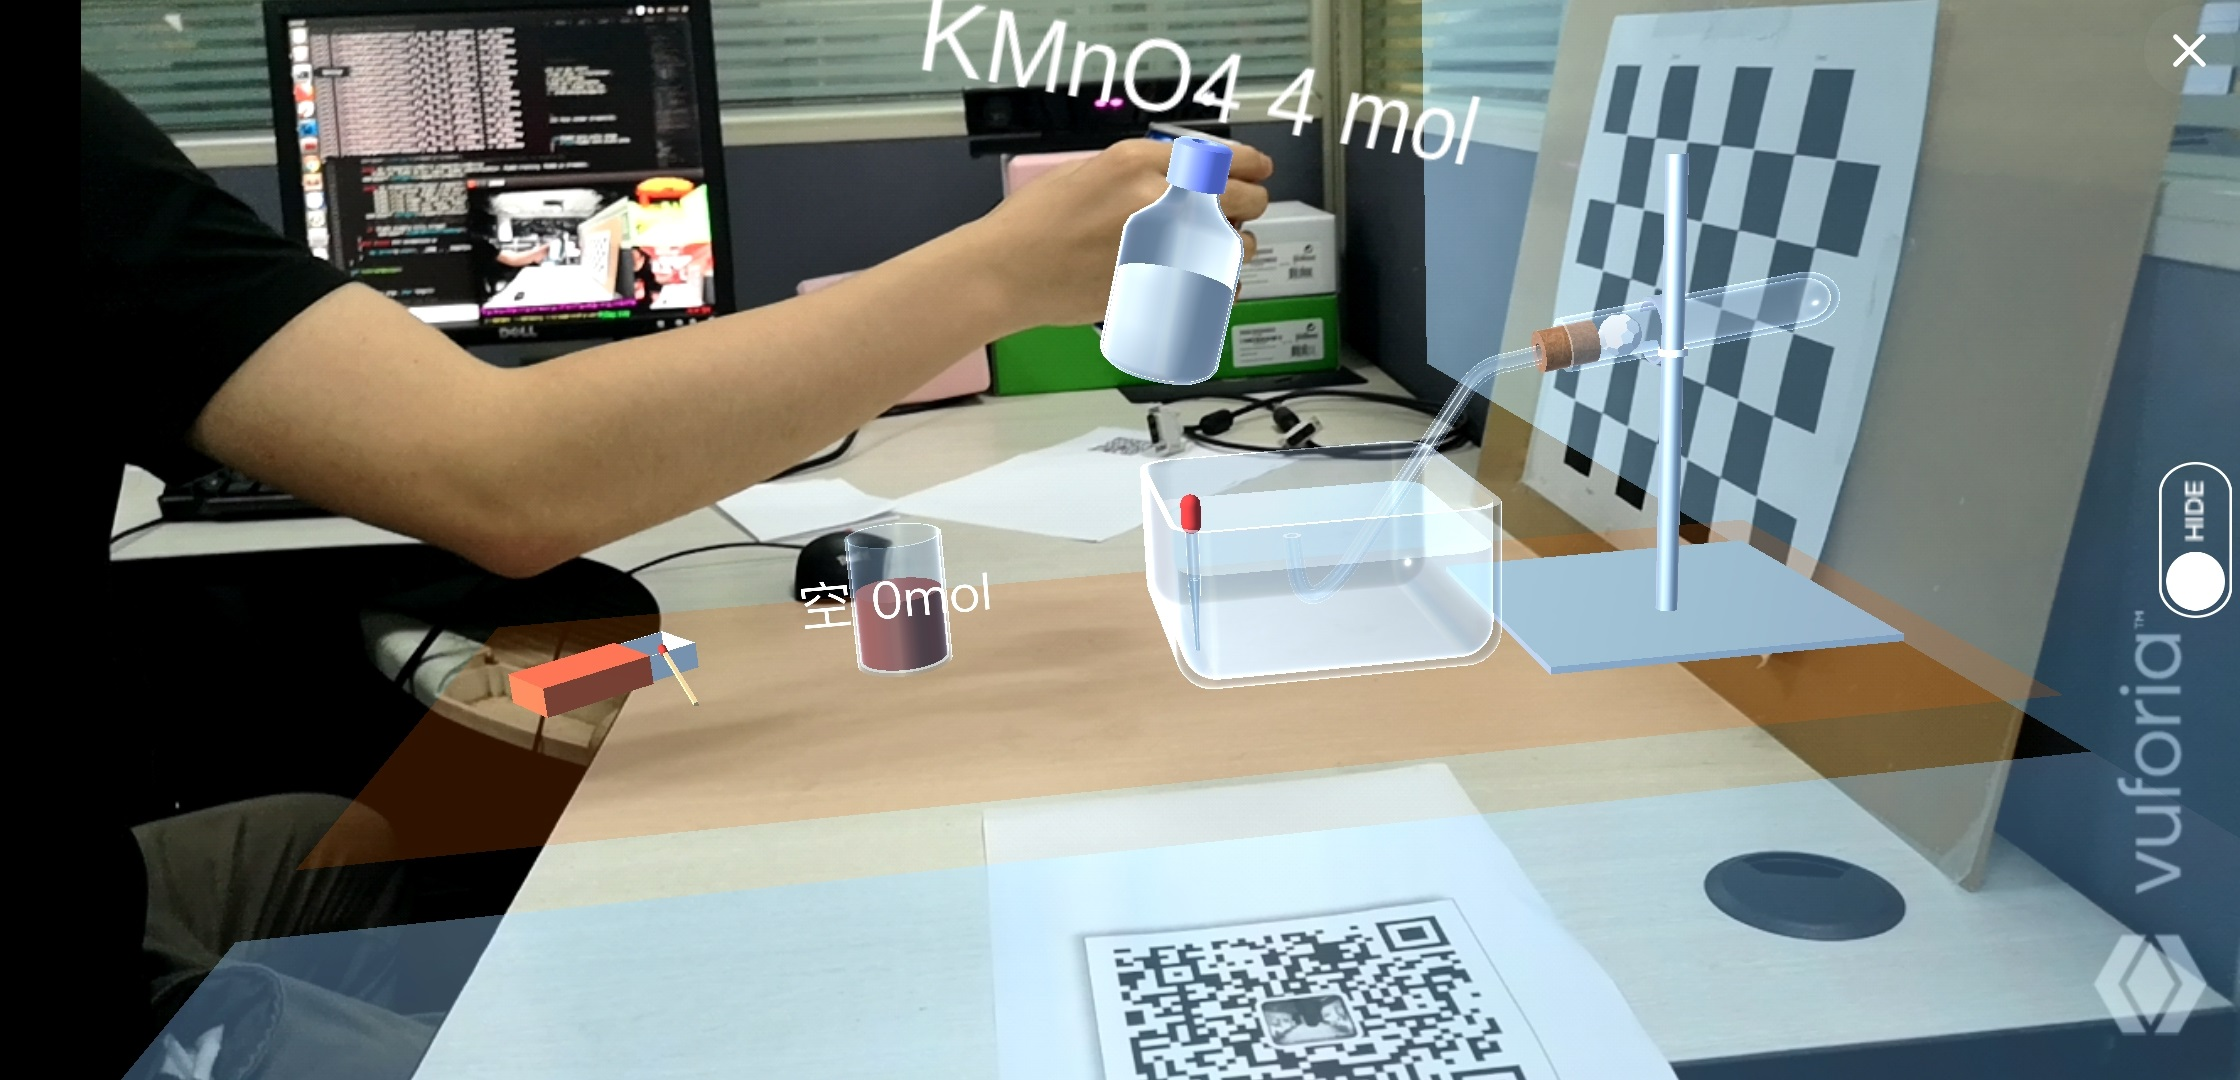
\includegraphics[width=12cm]{figure/moving.jpg}
  \bicaption[增强现实应用虚实融合和虚拟信息截图]
    {增强现实应用虚实融合和虚拟信息截图}
    {The Screen-shot of Virtual – Real Fusion and Virtual Hint Display in AR application }
 \label{fig:mAR}
\end{figure}

用户还可以切换被追踪物体的模型,例如烧杯、酒精灯、集气瓶等。在实现上述功能的基础上,本系统还提供了一些增强现实辅助实验的样例,例如酒精灯加热试管、集气瓶收集气体等。

\begin{figure}[!htp]
  \centering
  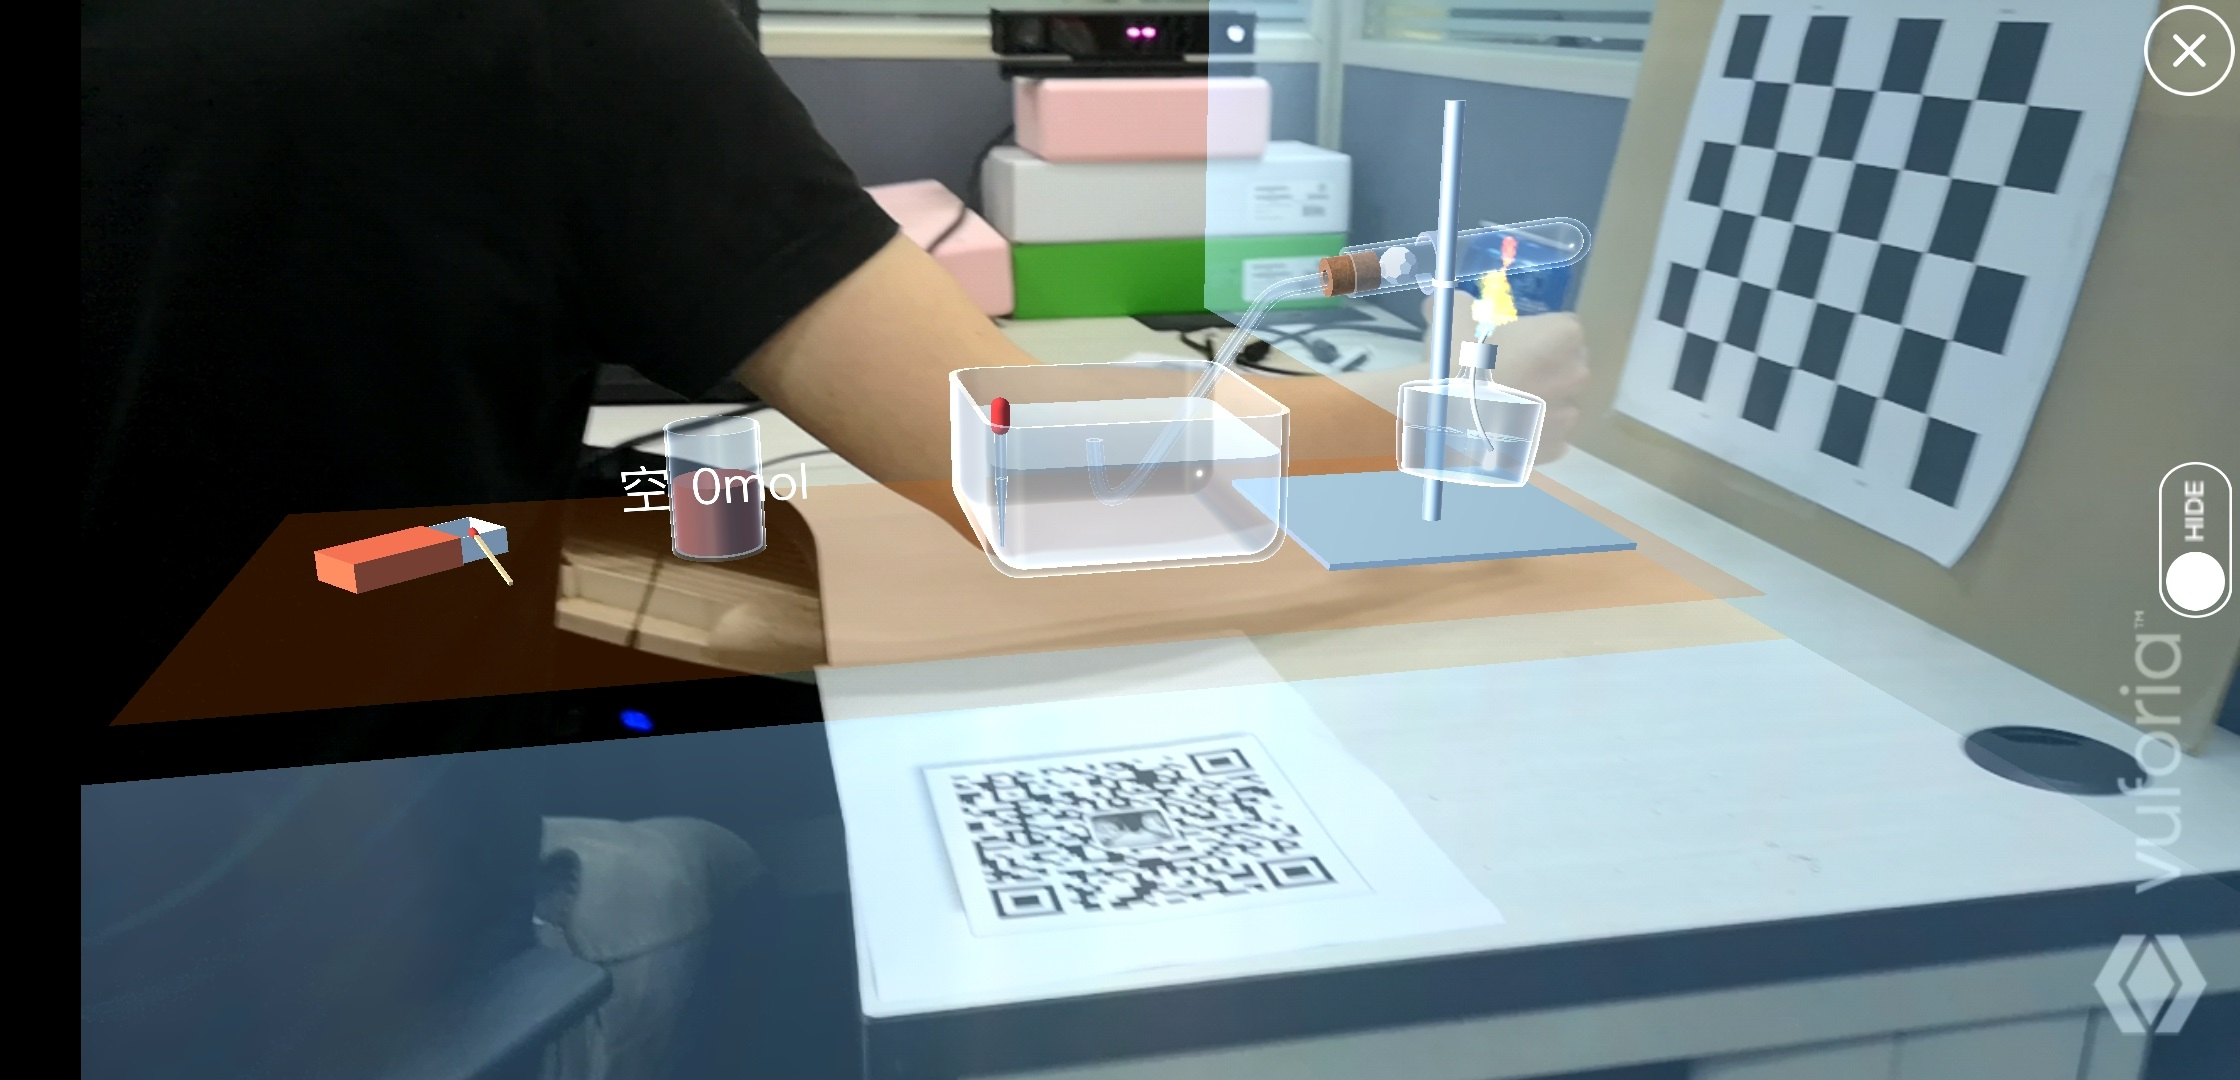
\includegraphics[width=6cm]{figure/heating.jpg}
    \hspace{1cm}
  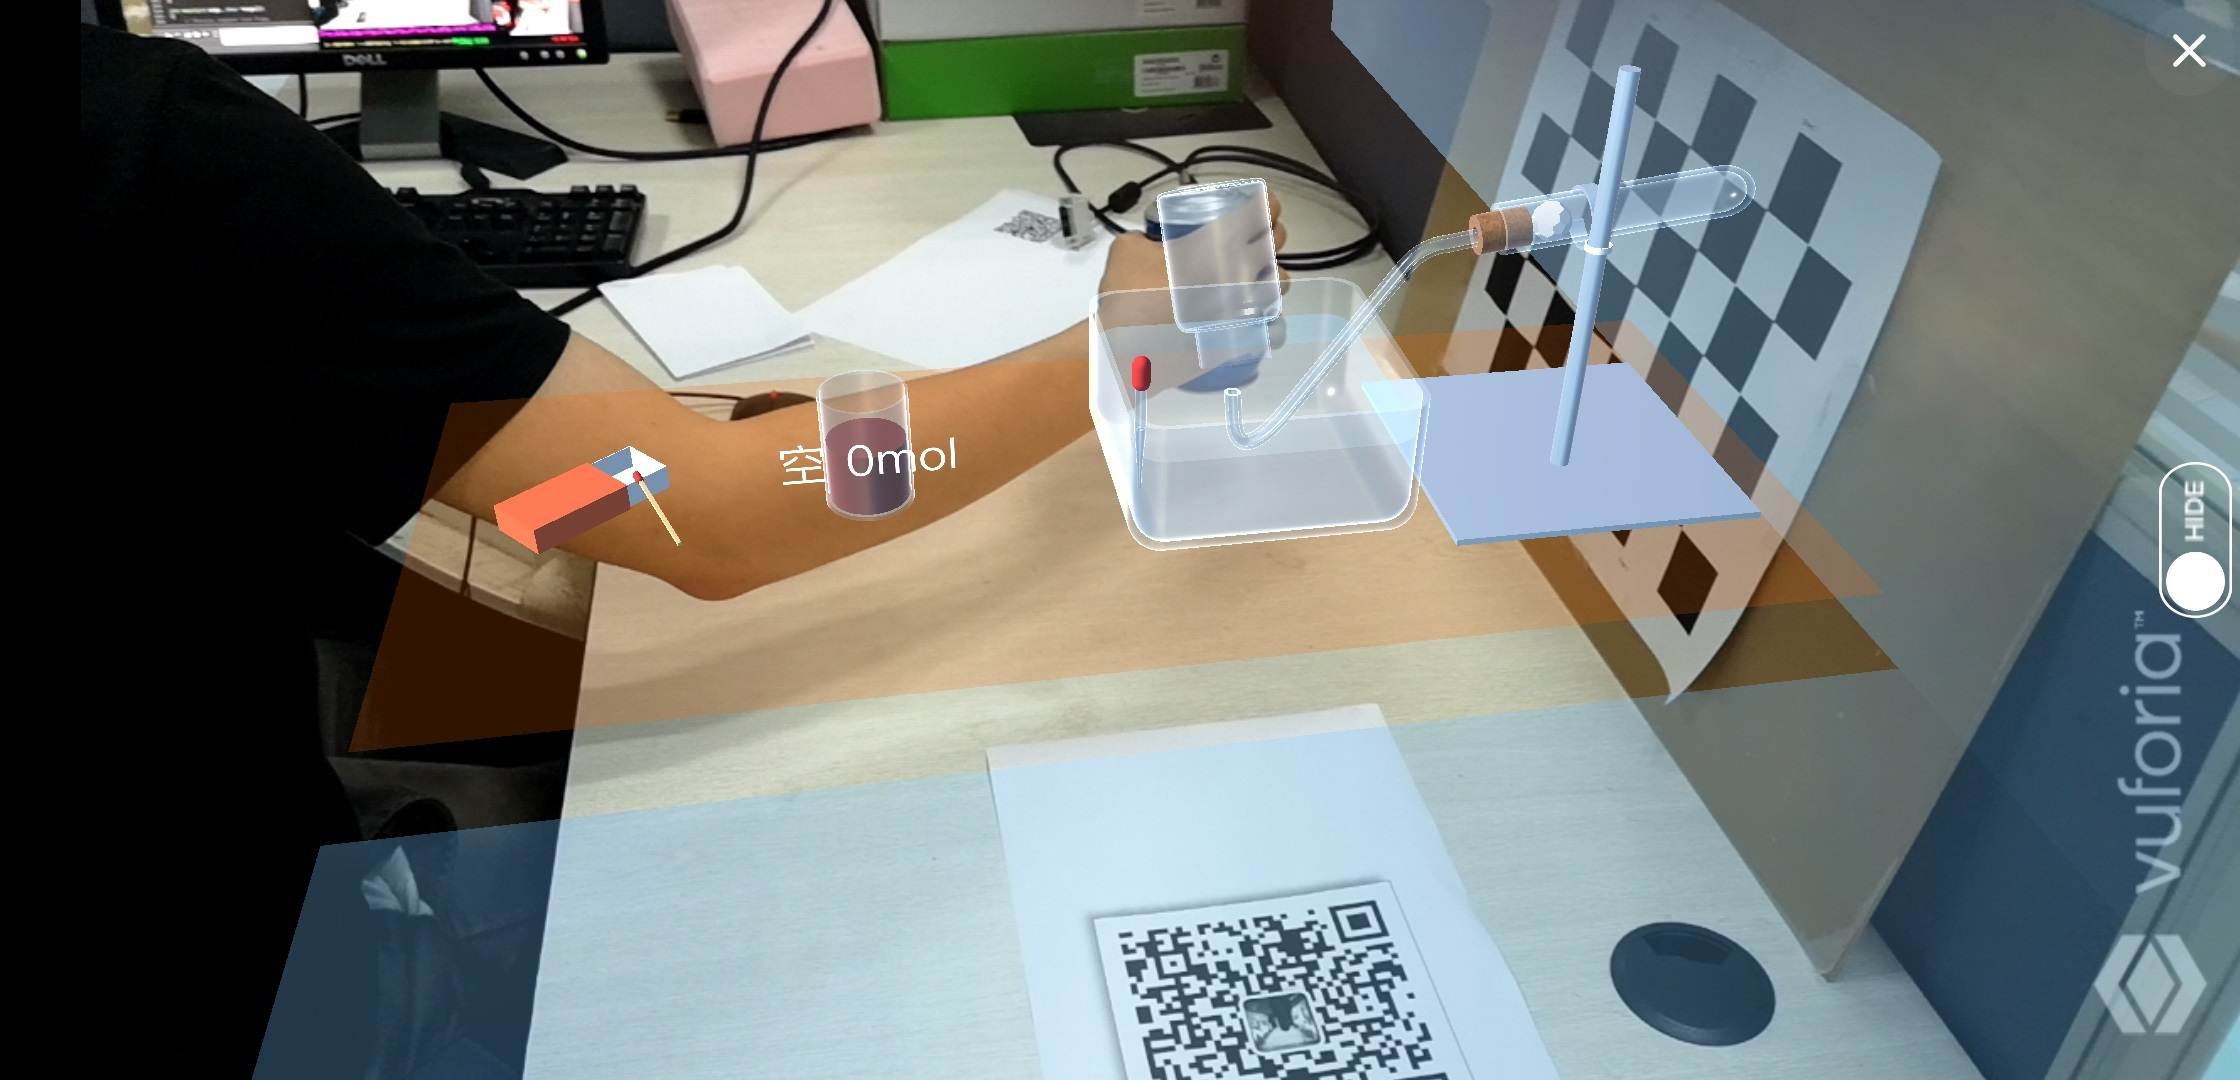
\includegraphics[width=6cm]{figure/gatheringGas.jpg}
  \bicaption[增强现实应用辅助实验样例图]
    {增强现实应用辅助实验样例图}
    {The Sample of Experimental Assistance in AR Application}
 \label{fig:comp}
\end{figure}

目前,场景中的虚拟物体与物体追踪服务器中得出的物体姿态数据保持一致。在比较精细的标定过程之后,也可以在手机屏幕上与真实物体融合得比较好。但是,由于Vuforia显示的虚拟物体是直接覆盖在摄像机图像上的,因此虚拟物体会覆盖在人手上,对于显示效果有一定的影响。

\section{本章小结}
本章对于物体追踪、网络传输的性能进行了一定的统计与分析,从软件层面和实际的应用体验来说,已经达到了预期要求。此外,也对客户端的编著、增强现实交互的体验进行了一些分析,一定程度上满足了用户需求。